Hemos probado entonces que nuestra matriz es banda 3,4. Sin embargo durante la aplicación 
de eliminación Gaussiana con pivoteo parcial eventualmente será necesario realizar intercambio de filas. 
Demostremos que luego de aplicar este método sobre una matriz banda $b_{p,q}$, la matriz resultante es banda $b_{p,(p+q)}$


\subsection{Demostración por inducción sobre el i-ésimo paso de la eliminación Gaussiana}

~

Sea $b_{p,q} \in R^{nxn}$, y sea $b^{i}$ la matriz resultante luego de aplicar el i-ésimo paso de eliminación Gaussiana con
pivoteo parcial. Probemos que al finalizar el método, la matriz $b^{n-1}$ obtenida es banda p, q+p.

~

\subsubsection{Caso base}

~

En el primer paso del método pueden suceder 2 cosas:

1) No se produce pivoteo sobre la primera fila $\Rightarrow$ demostración es trivial.

2) Se produce el intercambio entre la fila 1 y una fila $j$ con $1<j \leq (p+1)$. 

~

\underline{Bandas en la fila j al intercambiar fila 1 con fila j:}

La banda izquierda está determinada por la diferencia entre $j$ y la columna de menor índice que contenga un elemento distinto
de cero: llamemos a este índice $i$. Notemos que en el peor caso $i=1$ $\Rightarrow$ Banda izquierda = $j-i \leq (p+1) - i \leq
(p+1) - 1 = p$. (El máximo ancho de banda ''izquierda'' se produce al intercambiar la primera fila con la $p+1$.)

La banda derecha está determinada por la diferencia entre la columna de mayor índice $k$
que contenga un elemento distinto de cero y $j$ . Notemos que en el peor caso $j=2$ y $k =1+q$ $\Rightarrow$ Banda derecha =
$k-j \leq (1+q) -2 = (q-1)$. (El máximo ancho de banda ''derecha'' se produce al intercambiar la primera fila
con la segunda)

Por lo tanto la fila $j$ (en cualquiera de los casos) mantiene la propiedad de ser banda p,(p+q).

~

\underline{Bandas en la fila 1 al intercambiar fila 1 con fila j:}

Como estamos analizando la primera fila, es inmediato ver que la banda izquierda continúa siendo $p$, ya que no hay elementos
a la izquierda de la columna 1.

La banda derecha está determinada por la diferencia entre la columna de mayor índice $k$ que contenga un elemento distinto
de cero y la columna 1. Notemos que en el peor caso $j=1+p$ y $k=j+q$ $\Rightarrow k-1 = 1+p+q-1 = p+q$. (El máximo ancho de 
banda ''derecha'' se produce al intercambiar la primera fila con la $p+1$.)

Por lo tanto, la primera fila mantiene la propiedad de ser banda p,(p+q).

~

Sea $k$ una fila tal que $1 \leq k \leq (p+1)$. Luego de realizar el primer paso de Gauss y generar los ceros en la 
primera columna tenemos que:

- Banda izquierda de k $\leq (k-1) \leq (p+1)-1 = p$

- Banda derecha de k $ \leq (1+p+q)-k \leq p+q $

Como el resto de las filas no han sido modificadas, podemos afirmar que $b^{1}$ es banda p,(p+q). 
Demostrado caso base $\square$

~

\subsubsection{Paso inductivo: $P(i-1) \Rightarrow P(i)$}

~

Sea $j$ tal que $0 \leq j \leq (p-1)$. Analicemos brevemente qué sucede con cada una de las filas $i+j$.
En la matriz inicial $b^{0}$ sabíamos que el elemento más a la derecha para cada una de ellas estaba a lo sumo en la columna:
$i+j+q$. Sin embargo esta situación pudo haber cambiado luego de realizar el paso (i-1)-ésimo. En esta instancia, el
elemento más a la derecha podría estar a lo sumo en la columna: $i+p+q-1$. Notemos que $i+j+q \leq i+p+q-1 , \ \forall 
\ 0 \leq j \leq (p-1)$.

\begin{figure}[!h]
	\begin{center}
		  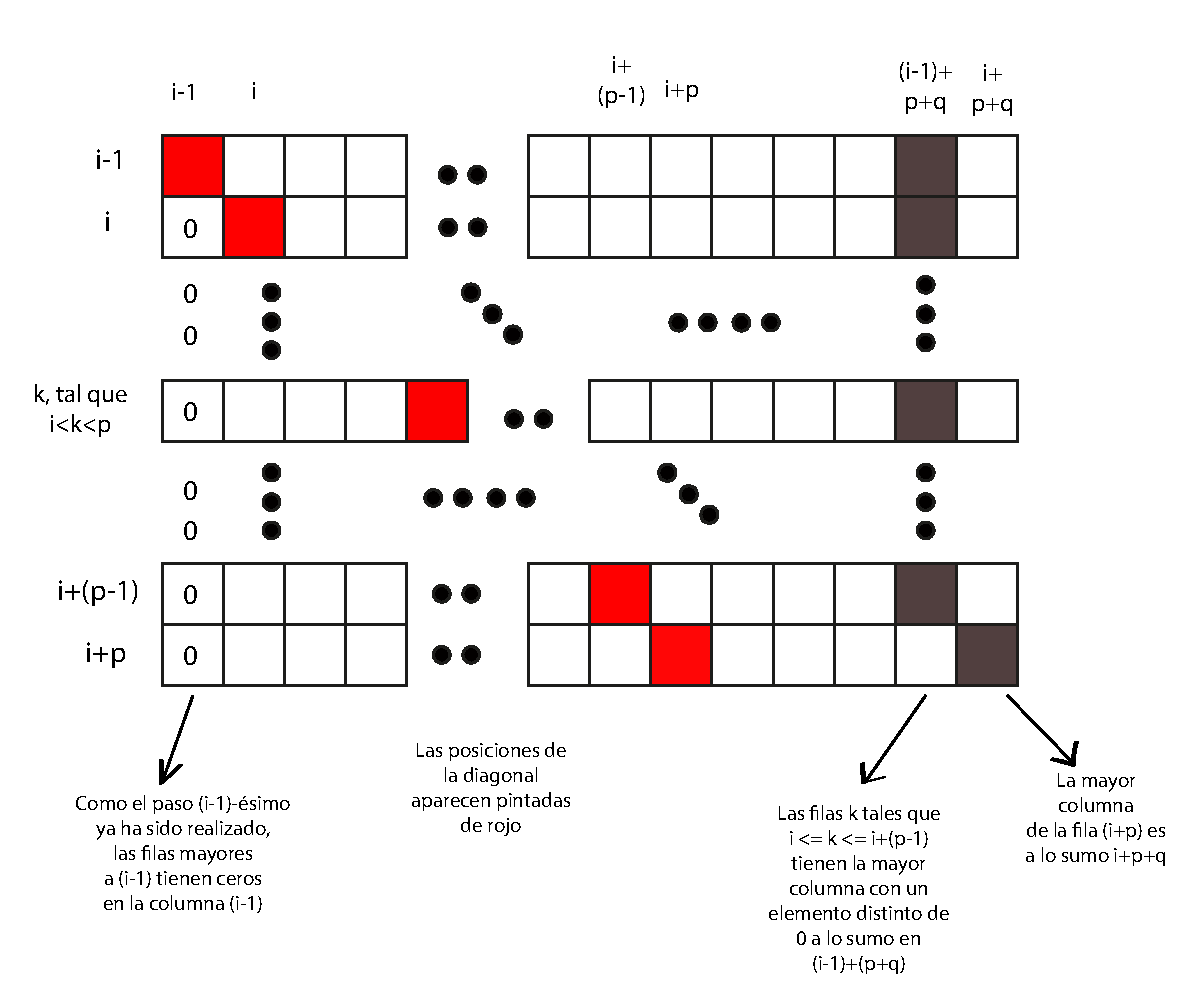
\includegraphics[scale=0.5]{Imagenes/im_8.pdf}
		  \caption{Estado de la matriz luego de realizar el (i-1)-ésimo paso. Se muestran únicamente
		  las filas y columnas que intervienen en el i-ésimo paso}
		  \label{fig:contra1}
	\end{center}
\end{figure}
\FloatBarrier

Para la fila $(i+p)$ la columna de mayor índice es a lo sumo $(i+p+q)$. Es suficiente probar que la matriz se mantiene como 
banda (p,p+q) luego de intercambiar las filas $i$ e $i+p$ ya que constituye el peor caso que podría ensanchar las bandas.

\begin{figure}[!h]
	\begin{center}
		  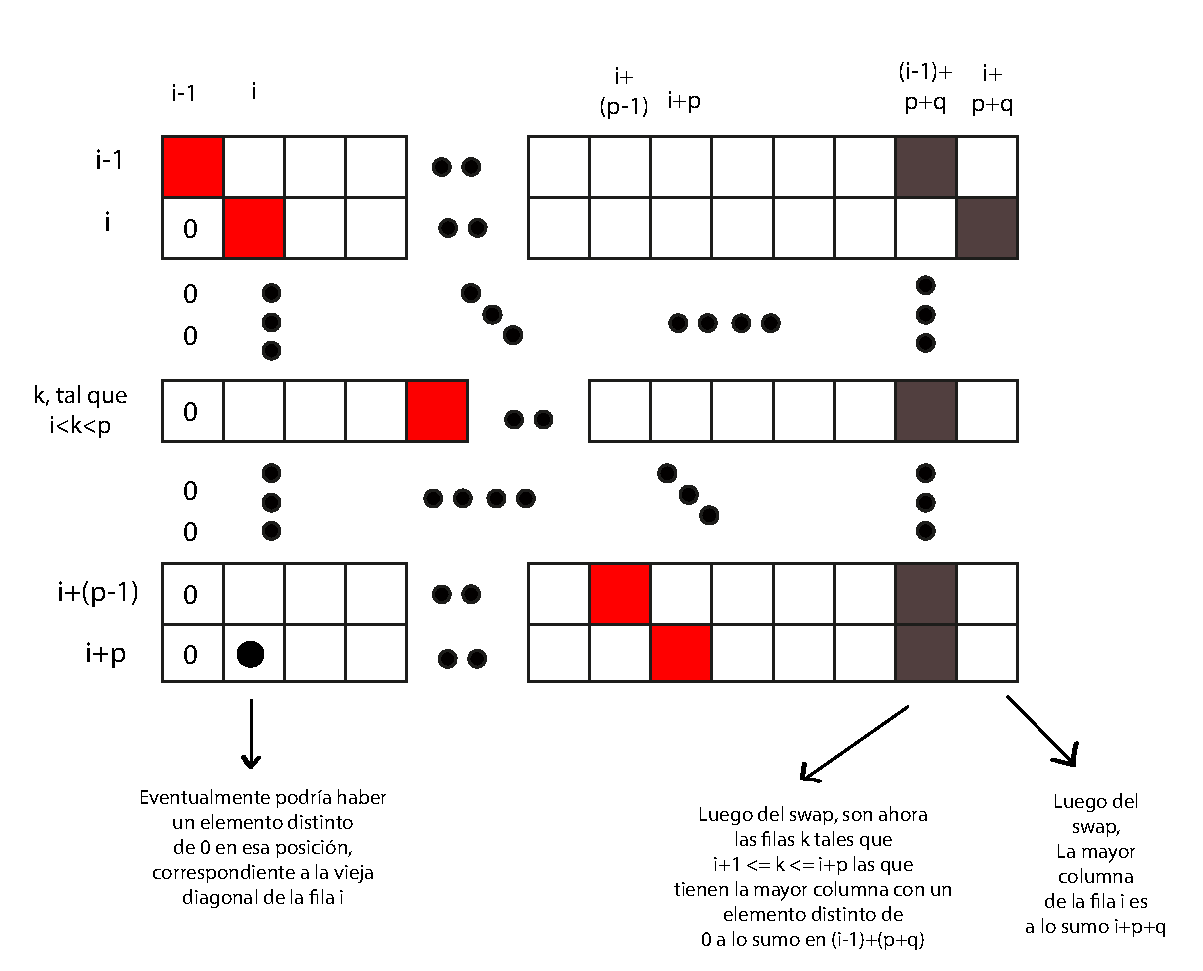
\includegraphics[scale=0.5]{Imagenes/im_9.pdf}
		  \caption{$b^{(i-1)}$ al swapear las filas i e (i+p), ya que constituye el peor caso que podría ensanchar
		  las bandas.}
		  \label{fig:contra1}
	\end{center}
\end{figure}

~

\underline{Bandas en la fila $i$ al intercambiar fila $i$ con fila $i+p$}

$Banda \ izquierda \leq i - (i+p-p) = 0$ (Columna de la diagonal menos columna del elemento más a la izquierda)

$Banda \ derecha \leq (i+p+q) - i = p+q$ (Columna del elemento más a la derecha menos columna diagonal)

La fila $i$ mantiene la propiedad de ser banda p,(p+q).

~

\underline{Bandas en la fila $i+p$ al intercambiar fila $i$ con fila $i+p$}

Como ya se han puesto ceros en las columnas a la izquierda de la i-ésima, tenemos que:

$Banda \ izquierda \leq (i+p) - (p) = 0$ (Columna de la diagonal menos columna del elemento más a la izquierda)

$Banda \ derecha \leq (i+p+q-1) - (i+p) \leq p+q$ (Columna del elemento más a la derecha menos columna diagonal)

La fila $(i+p)$ mantiene la propiedad de ser banda p,(p+q).

~

\begin{figure}[!h]
	\begin{center}
		  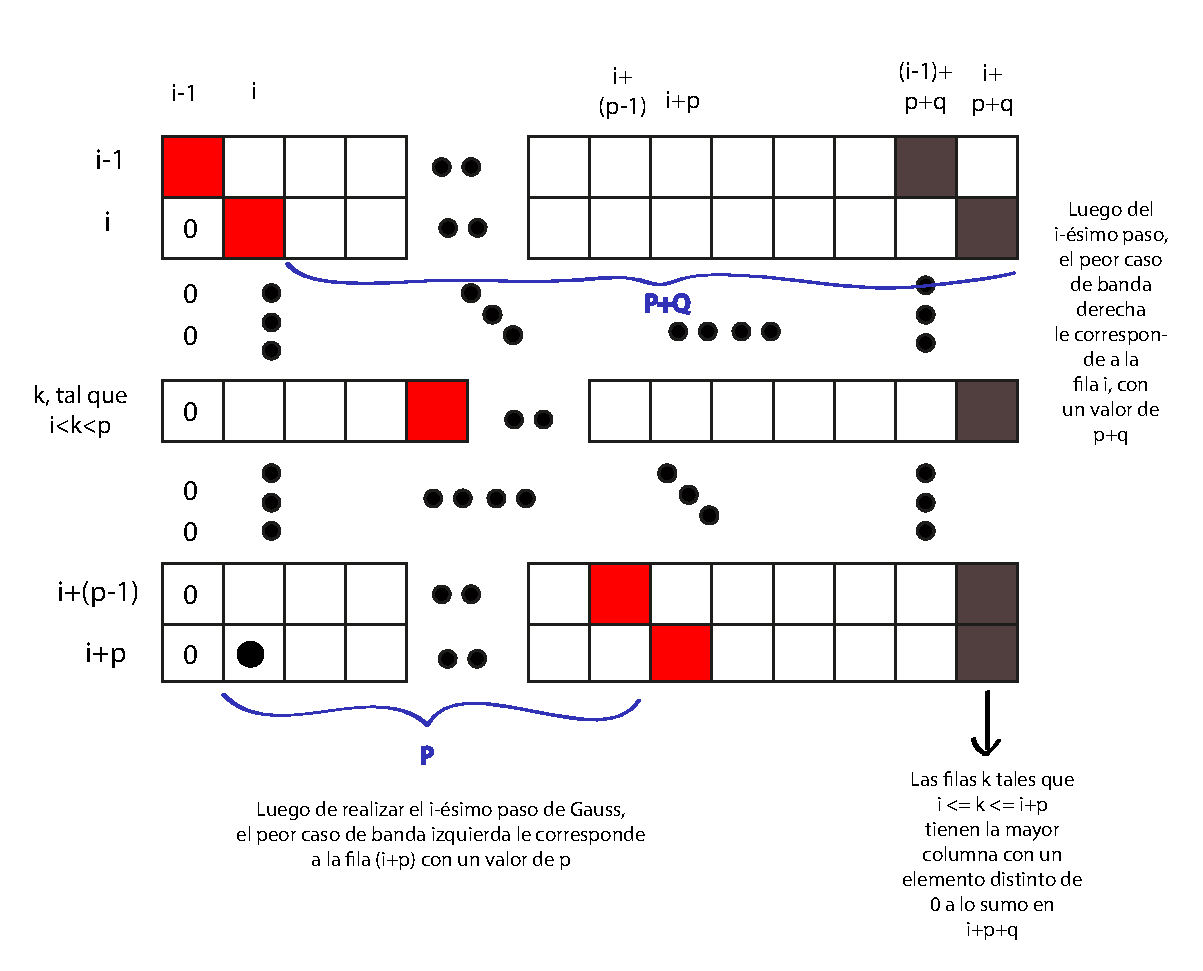
\includegraphics[scale=0.5]{Imagenes/im_10.pdf}
		  \caption{$b^{(i)}$ al realizar el paso habiendo intercambiado las filas i e (i+p)}
		  \label{fig:contra1}
	\end{center}
\end{figure}

Sea $k$ una fila tal que $i \leq k \leq (i+p)$. Luego de realizar el i-ésimo paso de Gauss y generar los ceros en la 
i-ésima columna tenemos que:

- Banda izquierda de k $\leq (k-i) \leq (i+p)-i = p$

- Banda derecha de k $ \leq (i+p+q)-k \leq (i+p+q)-i = p+q $

Como el resto de las filas no han sido modificadas, podemos afirmar que $b^{i}$ es banda p,(p+q). 
Demostrado paso inductivo $\square$

~

Aprovechando la propiedad que acabamos de mostrar, para almacenar nuestra matriz banda 3,(3+4) utilizamos una
matriz (en nuestro caso vector de vectores) de $4*n$ filas y 11 columnas. Inicialmente las diagonales corresponden
a la tercera columna de cada fila.

\begin{figure}[!h]
	\begin{center}
		  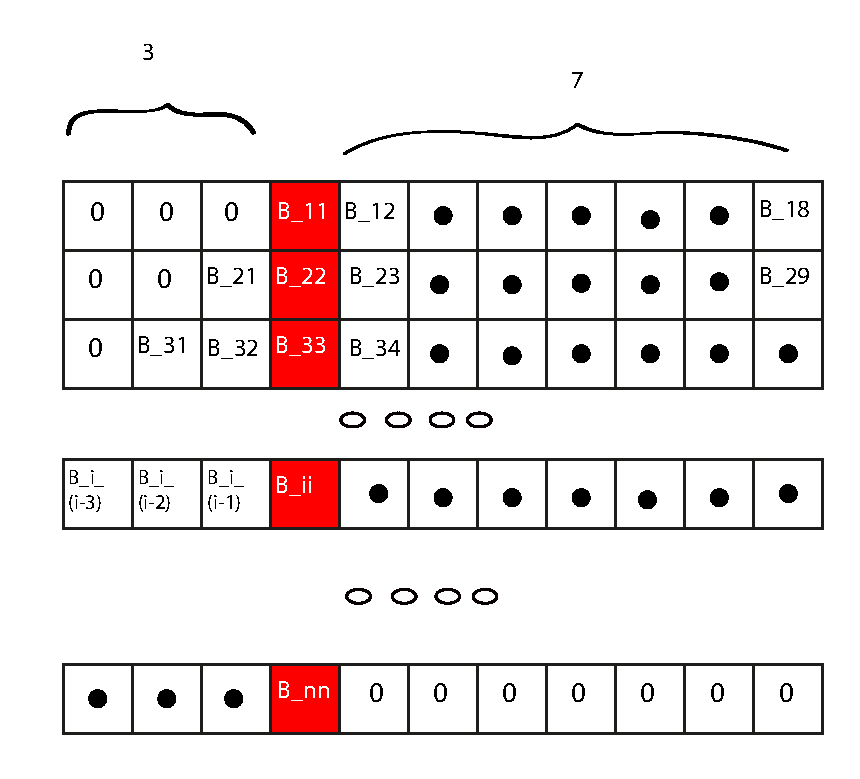
\includegraphics[scale=0.5]{Imagenes/im_13.pdf}
		  \caption{Representación de la matriz banda en nuestro código}
		  \label{fig:contra1}
	\end{center}
\end{figure}
\FloatBarrier
